\documentclass[twoside,twocolumn]{article}

\usepackage{blindtext} % Package to generate dummy text throughout this template 
\usepackage{graphicx}
\usepackage[sc]{mathpazo} % Use the Palatino font
\usepackage[T1]{fontenc} % Use 8-bit encoding that has 256 glyphs
\linespread{1.05} % Line spacing - Palatino needs more space between lines
\usepackage{microtype} % Slightly tweak font spacing for aesthetics

\usepackage[english]{babel} % Language hyphenation and typographical rules

\usepackage[hmarginratio=1:1,top=32mm,columnsep=20pt]{geometry} % Document margins
\usepackage[hang, small,labelfont=bf,up,textfont=it,up]{caption} % Custom captions under/above floats in tables or figures
\usepackage{booktabs} % Horizontal rules in tables

\usepackage{lettrine} % The lettrine is the first enlarged letter at the beginning of the text

\usepackage{enumitem} % Customized lists
\setlist[itemize]{noitemsep} % Make itemize lists more compact

\usepackage{abstract} % Allows abstract customization
\renewcommand{\abstractnamefont}{\normalfont\bfseries} % Set the "Abstract" text to bold
\renewcommand{\abstracttextfont}{\normalfont\small\itshape} % Set the abstract itself to small italic text

\usepackage{titlesec} % Allows customization of titles
\renewcommand\thesection{\Roman{section}} % Roman numerals for the sections
\renewcommand\thesubsection{\roman{subsection}} % roman numerals for subsections
\titleformat{\section}[block]{\large\scshape\centering}{\thesection.}{1em}{} % Change the look of the section titles
\titleformat{\subsection}[block]{\large}{\thesubsection.}{1em}{} % Change the look of the section titles

\usepackage{fancyhdr} % Headers and footers
\pagestyle{fancy} % All pages have headers and footers
\fancyhead{} % Blank out the default header
\fancyfoot{} % Blank out the default footer
\fancyhead[L]{Comparativa de Gestiores de BD NoSQL } % Custom header text
\fancyhead[R]{November 2020 } % Custom header text
\fancyfoot[RO,LE]{\thepage} % Custom footer text

\usepackage{titling} % Customizing the title section

\usepackage{hyperref} % For hyperlinks in the PDF

%----------------------------------------------------------------------------------------
%	TITLE SECTION
%----------------------------------------------------------------------------------------

\setlength{\droptitle}{-4\baselineskip} % Move the title up

\pretitle{\begin{center}\Huge\bfseries} % Article title formatting
\posttitle{\end{center}} % Article title closing formatting
\title{FORMAS DE EXTRACCIÓN DE DATOS NO ESTRUCTURADOS} % Article title
\author{Arias, Cancino, Crispin, Gutierrez, Zuñiga} 
\date{\today} % Leave empty to omit a date
\renewcommand{\maketitlehookd}{%
\begin{abstract}
	\begin{center}
		\textbf{Resumen}
	\end{center}
	La gestión de los datos no estructurados se ha convertido en uno de los principales retos a los que hacen frente las compañías en lo relativo a gestión de información y Big Data. En este documento damos una breve introducción al tratamiento de los mismos y las problemáticas más comunes en su gestión.
\\
	\begin{center}
		
		\textbf{Abstract}
	\end{center}
	The management of unstructured data has become one of the main challenges that companies face when it comes to information management and Big Data. In this document we give a brief introduction to their treatment and the most common problems in their management.
	\\
\end{abstract}
}
%----------------------------------------------------------------------------------------

\begin{document}
% Print the title
\maketitle
\vspace*{5 in}
\section{Introducción}
Un aumento voluminoso de datos no estructurados ha hecho que la gestión y extracción de datos sea un desafío, ya que los datos deben convertirse a formatos legibles por máquina para su análisis. Sin embargo, la creciente importancia de las decisiones basadas en datos ha cambiado la forma en que los gerentes toman decisiones estratégicas. Investigaciones muestra que las empresas que participan en la toma de decisiones basada en datos experimentan un crecimiento del 5 al 6 por ciento en su productividad.
\\
\section{Desarrollo}
\textbf{Definiciones de datos no Estructurados}
\\\\Una posible definición de datos no estructurados, son aquellos datos no almacenados en una base de datos tradicional. La información no estructurada no puede ser almacenada en estructuras de datos relacionales predefinidas.
Se pueden establecer diferentes clasificaciones, vamos a considerar dos de ellas.

\begin{itemize}
    \item Datos no estructurados y semiestructurados. Los datos semiestructurados serian aquellos datos que no residen de bases de datos relacionales, pero presentan una organización interna que facilita su tratamiento, tales como documentos XML y datos almacenados en bases de datos NoSQL.
    \item Datos de tipo texto y no texto. Datos no estructurados de tipo texto podría ser datos generados en las redes sociales, foros, emails, presentaciones Power Point o Documentos Word, mientras que datos no texto podrían ser ficheros de Imágenes jpeg, ficheros de audio mp3 o ficheros de video tipo flash.
\end{itemize}


\textbf{¿Qué es la extracción de datos? ¿Cómo puede ayudar a las empresas?}\\

En términos simples, la extracción de datos es el proceso de extraer datos capturados dentro de fuentes semiestructuradas y no estructuradas, como correos electrónicos, PDF, formularios PDF, archivos de texto, redes sociales, códigos de barras e imágenes. ¿Cómo se realiza la extracción de datos? Una herramienta de extracción de datos de nivel empresarial hace que los datos comerciales entrantes de fuentes no estructuradas o semiestructuradas se puedan utilizar para análisis de datos e informes.\\

\textbf{Extracción de datos Vs Minería de datos}\\
\\La gente a menudo confunde extracción de datos y minería de datos. La extracción de datos se ocupa de la información existente para su posterior procesamiento, mientras que la minería de datos es un proceso que se utiliza para buscar patrones, anomalías y correlaciones en sus datos. Por lo tanto, una herramienta de minería de datos permite a los usuarios analizar datos desde múltiples perspectivas para identificar patrones ocultos en grandes conjuntos de datos.
\\

\textbf{¿Pueden aprovecharse los datos no estructurados? }\\
\\Extraer información útil de datos no estructurados presenta un mayor desafío que hacerlo de datos estructurados, sin embargo, es posible explotar esta información. El análisis de cada tipo de dato no estructurado es en sí una disciplina distinta: 
\\Texto: natural language processing (NLP) / text mining. 
\\Habla: speech technologies / NLP. 
\\Imágenes / video: image processing
\\Aplicaciones: Texto
\\Análisis de sentimiento
\\Ejemplo: Hedenometer
\\
\begin{center}
	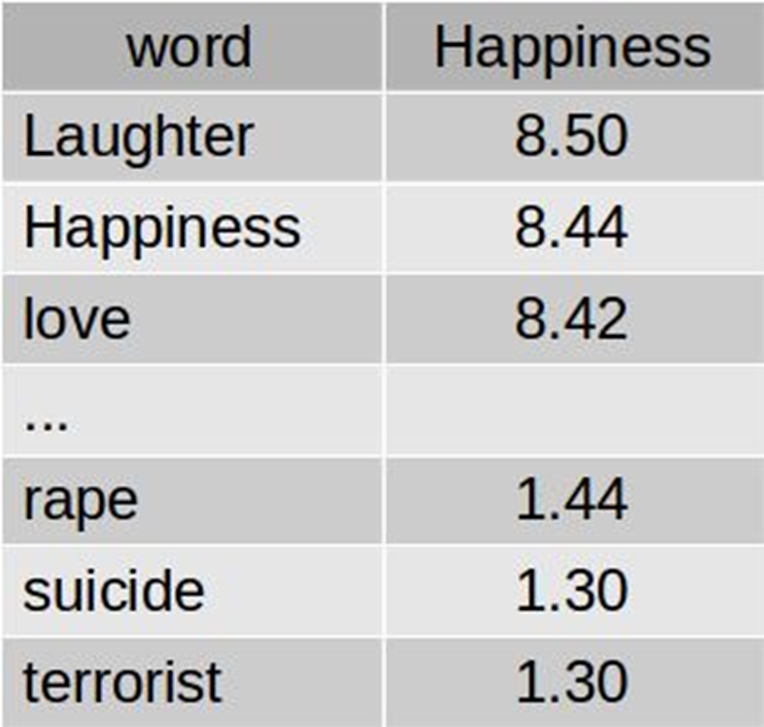
\includegraphics[ width=5cm]{./img/bd1.png} 
\end{center}
\begin{center}
	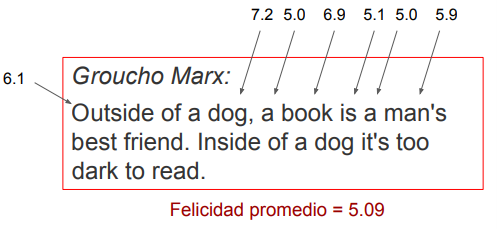
\includegraphics[ width=6cm]{./img/bd2.png} 
\end{center}
Léxico de felicidad para twitter
\begin{center}
	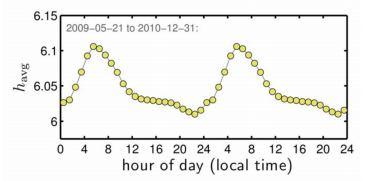
\includegraphics[ width=6cm]{./img/bd3.png} 
\end{center}


\textbf{Aplicaciones: habla}\\
\\Modelando la relación entre audio y palabras dichas se pueden implementar sistemas que hagan las siguientes tareas:\\
\begin{itemize}
    \item Automatic speech recognition	(nos permite pasar al análisis de texto).
    \item Speech synthesis.
\end{itemize}
Componentes claves detrás de los asistentes	virtuales (Google Assistant, Siri, Alexa, Cortana, etc.)
\\Pero ojo, el habla es más que sólo la transcripción del texto,  posee también características prosódicas que hacen al  mensaje. Por ejemplo:
\begin{itemize}
    \item Tono / frecuencia.
    \item Velocidad del habla.
    \item Intensidad del habla.
    \item Calidad del habla.
\end{itemize}
Esto se analiza en tiempo real en los sistemas de diálogo (por ejemplo para cambios de turnos).\\
\begin{center}
	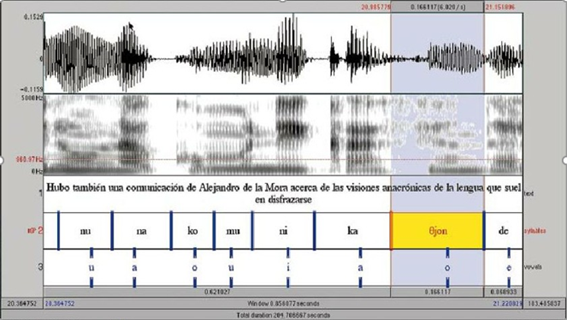
\includegraphics[width=5cm]{./img/bd4.png} 
\end{center}

\textbf{Aplicaciones: imágenes}\\
\begin{center}
	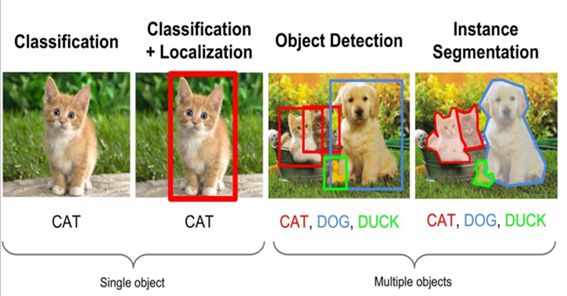
\includegraphics[width=6cm]{./img/bd5.png} 
\end{center}
Clasificacion en imágenes
\begin{center}
	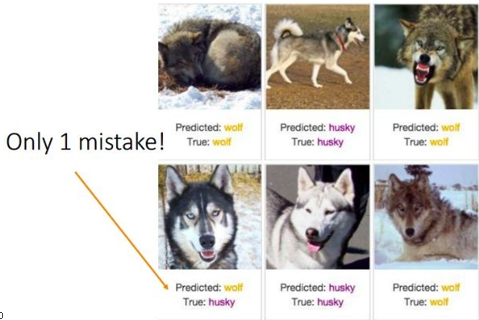
\includegraphics[width=6cm]{./img/bd6.png} 
\end{center}

\textbf{Aplicaciones: videos}\\
\begin{center}
	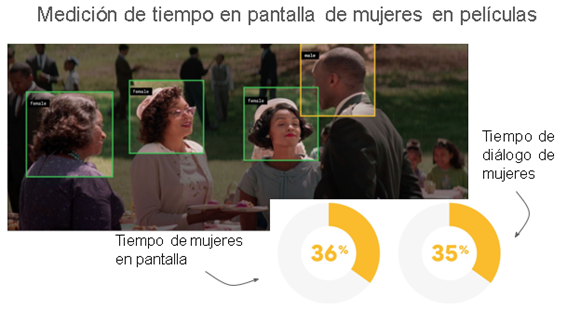
\includegraphics[width=6cm]{./img/bd7.png} 
\end{center}

\textbf{Ejemplo sencillo tratamiento de datos no estructurados (redes sociales)}\\
Dada la variada naturaleza de los datos no estructurados, hay infinidad de posibles procesos relacionados con ellos. A continuación, mostramos un sencillo ejemplo de tratamiento de datos provenientes de redes sociales.
El objetivo de este análisis de datos es conocer la percepción que existe el precio de determinado producto de twitter.
\begin{itemize}
    \item Extraccion: Utilizadno una clase de java(ejemplo twitter 4j) leemos el feed de Twitter disponible en https://twitter.com/search/realtime. Añadimos a los campos disponibles calificaciones del tipo: idioma, localización geográfica.
    \item Transformacion: Filtramos todos aquellos tuits que contengan el nombre del producto. Refinamos el filtro introduciendo campos del tipo (“precio”) + (“barato”,”caro”,”economico”,etc…),teniendo en cuenta el idioma en el que se generan los tuits.
    \item Valorar la opción en base al volumen de obtener una muestra representativa de los datos extraidos y filtrados.
    \item Volcado a BBDD:Insertamos en una tabla el registro del tuit con la calificación identificada(idioma , locaclizacion geografica)
    \item Informes: Creamos informe que permita realizar análisis por tiempo y campos de calificación. Hay que considerar que este informe puede ser actualizado en tiempo real.
\end{itemize}


\section{Conclusiones}
\begin{itemize}
    \item No sólo los datos estructurados pueden ser analizado. 
    \item Hay una gran disponibilidad de datos no estructurados. 
    \item Existen múltiples técnicas para analizar distintos tipos de datos no estructurados. 
    \item Hoy en día se están haciendo grandes avances en esta línea.
\end{itemize}

\section{Recomendaciones}
Aprender y practicar mucho programar y manejar estructuras de datos  eficientes.


\section{Biblografia}

\begin{itemize}
    \item CS231n Convolutional Neural Networks for Visual Recognition. (2021). Retrieved 6 January 2021, from https://cs231n.github.io/classification/ 
    \item Using technology to address gender bias in film - Google. (2021). Retrieved 6 January 2021, from https://about.google/intl/en/main/gender-equality-films/
    \item Ahmed, I. (2021). Herramientas de extracción de datos: alcance las perspectivas más rápido | Astera. Retrieved 6 January 2021, from https://www.astera.com/es/tipo/blog/\\Herramientas-automatizadas-de-extracci\%C3\%B3n-de-datos-para-una-comprensi\%C3\%B3n-m\%C3\%A1s-r\%C3\%A1pida./
    http://www.wrox.com/WileyCDA/WroxT\\itle/Professional-NoSQL.productCd-047094224X.html 
    \item Gestión de datos no estructurados: ¿cómo extraer información relevante?. (2021). Retrieved 6 January 2021, from https://www.astera.com/es/tipo/blog/\\gesti\%C3\%B3n-de-datos-no-estructurados/
    http://revistas.udistrital.edu.co/ojs/index.\\php/tia/article/viewFile/8769/pdf
    \item Tipos de datos: datos estructurados, semiestructurados y no estructurados. (2021). Retrieved 6 January 2021, from https://blogs.imf-formacion.com/blog/tecnologia/tipos-de-datos-datos-estructurados-semiestructurados-y-no-estructurados-202006/
    \item Arias, W. (2021). BIG DATA: EXTRAER, TRANSFORMAR Y CARGAR LOS DATOS - Instituto Internacional de Ciencia de Datos. Retrieved 6 January 2021, from https://i2ds.org/2016/05/04/big-data-extraer-transformar-y-cargar-los-datos/
\end{itemize}

%%%%%%%%%%%%%%%%%%%%%%%%%%%%%%%%%%%%%%%%%%%%%%%%%%%%%%%%%
\end{document}